\section{System enviroment configuration}
	\subsection{IntelliJ IDEA integrated development environment configuration}
	Per una corretta configurazione di IntelliJ IDEA è necessario configurare i path di sistema\glo e importare un progetto esistente.
	
	A correct IntelliJ IDEA configuration needs to configure the path system\glo and after that to import an existing project.
	
	\begin{figure}[H]
		\centering
		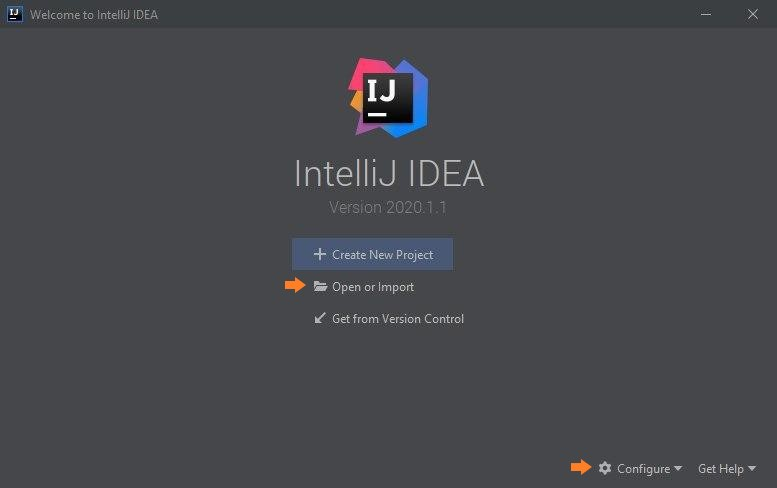
\includegraphics[scale=0.70]{../Developer_manual/img/intellijidea_main.jpg}
		\caption{IntelliJ IDEA first execution}
	\end{figure}	

	

	\subsubsection{Path system configuration}
	Una volta avviato IntelliJ IDEA spostarsi su "Configure" | "Settings" in basso a destra. Dopo aver inserito "Node.js and NPM" nella barra di ricerca verificare che i campi "Node interpreter" e "Package manager" siano impostati correttamente, altrimenti aggiornare i percorsi selezionando la cartella corretta.
	
	Once you run IntelliJ IDEA move to "Configure" then "Settings"in the lower-right corner. Write "Node.js and NPM" in the search bar and check for the correct settings of fields "Node interpreter" and "Package manager", oherwise update them with the correct paths. 

\begin{figure}[H]
		\centering
		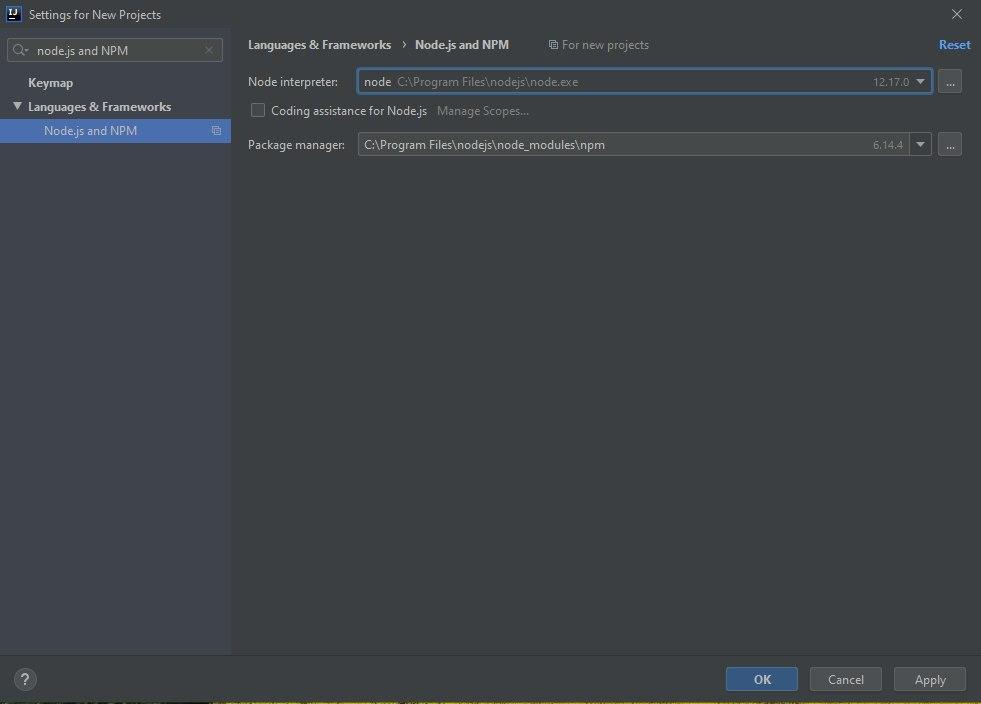
\includegraphics[scale=0.60]{../Developer_manual/img/nodejs_and_npm.jpg}
		\caption{Node.j and NPM settings}
	\end{figure}	

	\subsection{Project import}
	Dalla schermata principale cliccare la voce "Open or Import" e selezionare la root directory del repository contenente il nostro progetto.

	From IntelliJ IDEA main window click on "Open or Import" and select the root directory of our project repository folder.

\begin{figure}[H]
		\centering
		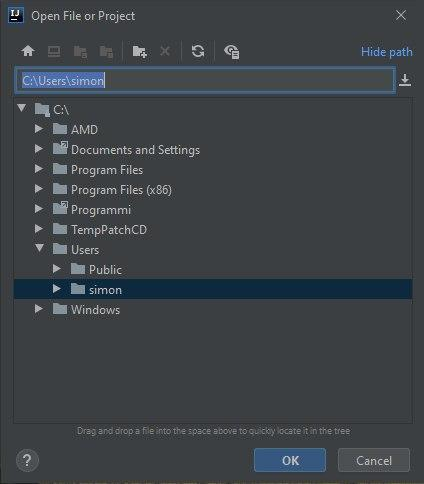
\includegraphics[scale=0.80]{../Developer_manual/img/open_project.jpg}
		\caption{Project path on opening}
	\end{figure}	


	\subsection{ESLint configuration}
		\subsubsection{Automatic configuration}
	Se ESLint è presente tra le dipendenze del progetto, viene configurato in automatico da IntelliJ IDEA. Verificare che sia attivo andando su "File" | "Settings" | "Languages and Frameworks" | "JavaScript" | "Code Quality Tools" | "ESLint" e controllare che sia selezionata la checkbox di configurazione automatica. 
	
When ESLint is listed as a dependency in our project IntelliJ IDEA automatically configures it. Move to "File" | "Settings" | "Languages and Frameworks" | "JavaScript" | "Code Quality Tools" | "ESLint" and check that Automatic ESLint configuration option is enabled. 


\begin{figure}[H]
		\centering
		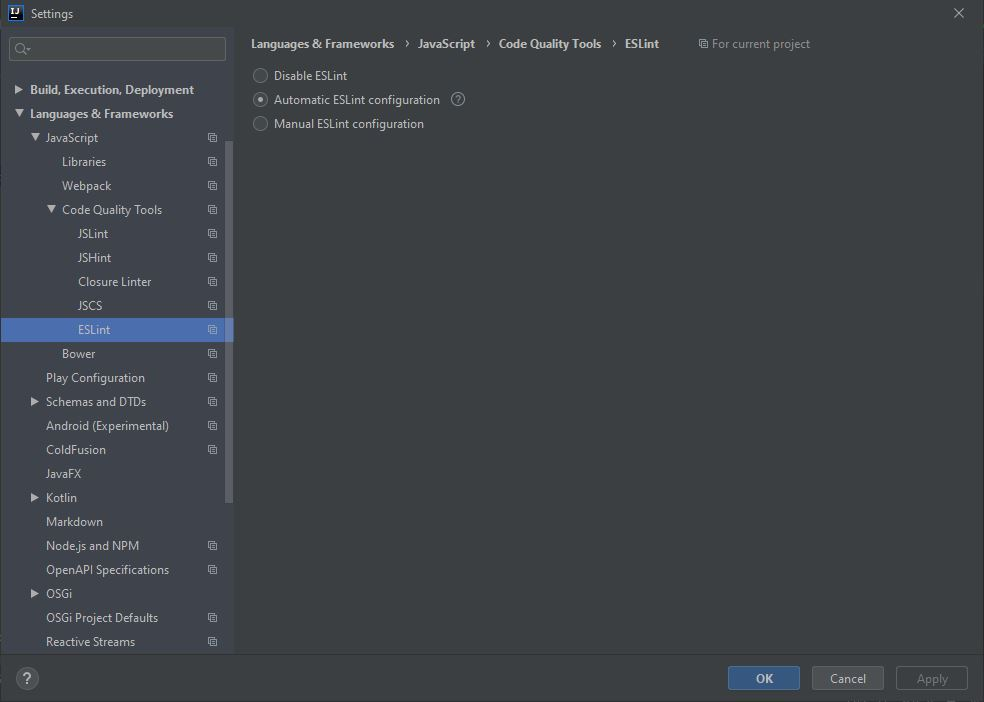
\includegraphics[scale=0.60]{../Developer_manual/img/automatic_eslint_configuration.JPG}
		\caption{Automatic ESLint configuration}
	\end{figure}	

		\subsubsection{Manual configuration}
	
	Se lo sviluppatore lo desidera può configurare ESLint manualmente selezionando la checkbox di configurazione manuale e procedendo come segue: 
	\begin{enumerate}
		\item inserire il path di Node.js nel campo "Node interpreter";
		\item nel campo "ESLint package" specificare la posizione del package eslint o dello standard package;
		\item scegliere il file di configurazione decidendo se affidare a IntelliJ IDEA la ricerca in modo automatico oppure selezionando un percorso a tale file. 
		\item opzionalmente compilare i campi "Additional Rules Directory" per specificare un ulteriore command-line per ESLint e  "Extra ESLint Options" per specificare la posizione di file con ulteriori configurazioni e confermare.
	\end{enumerate}
		
		You can also configure ESLint manually checking the Manual ESLint configuration option and complete fields as it follows:
		\begin{enumerate}
			\item in the "Node Interpreter" field, specify the path to Node.js;
			\item in the "ESLint Package" field, specify the location of the eslint or standard package;
			\item choose the configuration file to use checking "Automatic search" if you want to let IntelliJ IDEA do it for you or specify the file location in the path field;
			\item optionally specify additional command-line options to run ESLint in "Extra ESLint Options" field and specify the location of the files with additional code verification rules in the "Additional Rules Directory" field then confirm the whole configuration.
		\end{enumerate}
		

\begin{figure}[H]
		\centering
		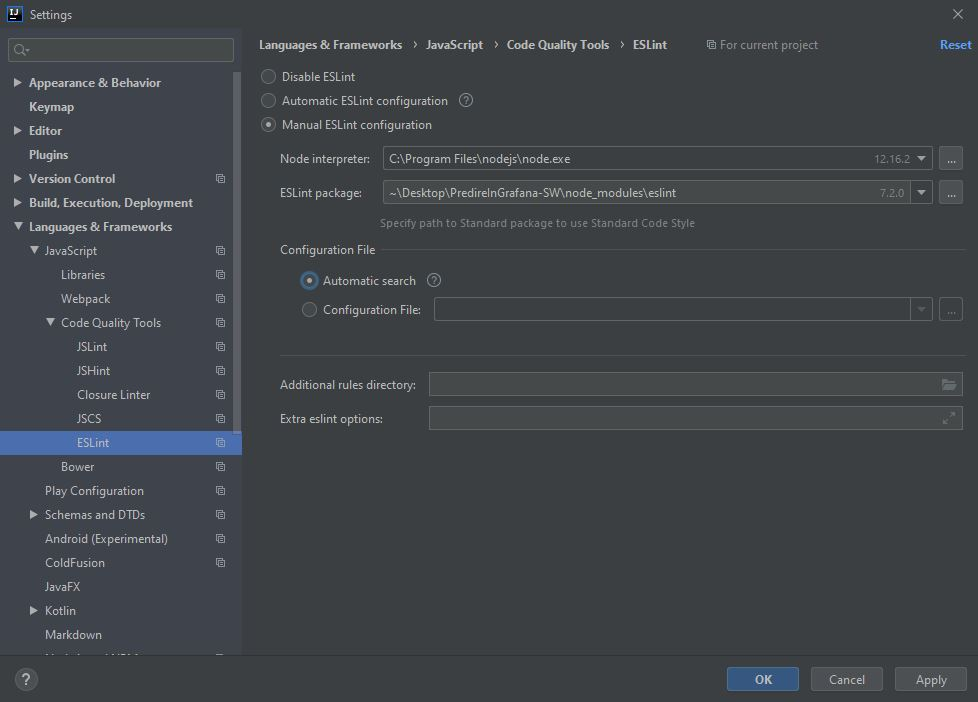
\includegraphics[scale=0.60]{../Developer_manual/img/manual_eslint_configuration.JPG}
		\caption{Manul ESLint configuration}
	\end{figure}	

	
	\subsection{Grafana plugin panel enviroment configuration}
	
	
		\subsubsection{package.json content}
		Nel file package.json si trovano tutte le informazioni e i requisiti necessari al corretto funzionamento della nostra applicazione. Di seguito la lista degli attributi che rappresentano le informazioni più importanti:
		\begin{itemize}
			\item\textbf{scripts}: contiene una lista dei comandi usati dallo sviluppatore eseguibili da linea di comando:
			\begin{itemize}
				\item build:
				\item test:
				\item dev:
				\item watch:
			\end{itemize}

			\item\textbf{dependencies}: contiene i seguenti pacchetti necessari al corretto funzionamento della nostra applicazione:
			\begin{itemize}
			 	\item @influxdata/influxdb-client: il client javascript di riferimento per InfluxDB. Sono supportati gli ambienti node e browser;
    			\item axios: client HTTP per browser e Node.js;
    			\item react-files: componente React per la gestione di file di input (dropzone) usato nel caricamento dei file JSON all'interno del plugin.
			\end{itemize}
			\item\textbf{devDependencies}: contiene i seguenti pacchetti necessari al corretto funzionamento della nostra applicazione durante lo sviluppo:
				\begin{itemize}
					\item @grafana/data: libreria che contiene la maggior parte delle funzionalità di base e i tipi di dato utilizzati dalla piattaforma Grafana;
					\item @grafana/toolkit: CLI che semplifica e aumenta l'efficienza dello sviluppo di un plugin in Grafana;
					\item @grafana/ui: libreria che contiene i differenti componenti di design della piattaforma Grafana;
					\item webpack: usato per compilare i moduli JavaScrip. Con webpack lo sviluppatore può interfacciarsi sia da riga di comando che da API.
				\end{itemize}
				
		\end{itemize}
		
		In package.json file you can find all the app informations and requirements needed for its proper functioning. Attributes which represent important information are listed below:
		\begin{itemize}
			\item\textbf{scripts}: it contains all CLI command lines used from the developer: 
				\begin{itemize}
				\item build:
				\item test:
				\item dev:
				\item watch:
			\end{itemize}
			\item\textbf{dependecies}: it contains the following packages needed for our app proper functioning:
			\begin{itemize}
				\item @influxdata/influxdb-client: the reference javascript client for InfluxDB. Both node and browser environments are supported;
    			\item axios: promise based HTTP client for the browser and node.js;
    			\item react-files: a file input (dropzone) management component for React we use when loading JSON files.
			\end{itemize}
			\item\textbf{devDependencies}: it contains the following packages needed for our app proper functioning during development:
			\begin{itemize}
				\item @grafana/data: a library containing most of the core functionality and data types used in Grafana.
				\item @grafana-toolkit: a CLI\glo that enables efficient development of Grafana plugins.
				\item @grafana/ui: a library containing the different design components of the Grafana ecosystem;
				\item webpack: used to compile JavaScript modules. Once installed, you can interface with webpack either from its CLI or API.
			\end{itemize}
		\end{itemize}
	